\chapter{Results} \label{ch:conclusions}

In order to determine the effectiveness of the GPU-based FDTD implementation, we compare performance of GPU and CPU implementations. Performance is measured as a function of total execution time for a given domain size, as well as throughput (cells updated per second).

\section{Test Environment}

Tests were performed on a 2015 Dell XPS 9550 with 32GB of RAM, Intel i7 2600 CPU and NVIDIA 960M GPU. GoLightly GPU tests were executed under Microsoft Windows 10, while Meep CPU tests were run under Ubuntu Desktop version 16.04.   \footnote{Meep is incompatible with Microsoft Windows. Thus, Ubuntu was used for the CPU simulation, while the GPU simulation was benchmarked in its target Microsoft Windows environment.}

\section{Performance Metrics}

Metrics were calculated using domain sizes ranging from 128x64 to 8192x4096 over 5000 frames. (In this case, a frame represents a complete time step wherein both E and H fields are updated.) For benchmarking purposes, the visualizer was disabled.


\begin{figure}[H]
	\centering
	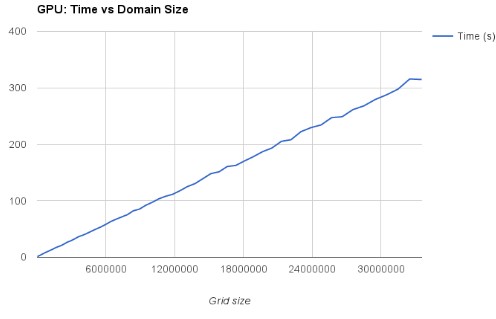
\includegraphics[width=\textwidth,
	keepaspectratio]{gpu_time_vs_domain_size.png}
	\caption{GoLightly: seconds for 5000 frames with the given domain size}
	\label{fig:gpuTimeVsDomainSize}
\end{figure}

\autoref{fig:gpuTimeVsDomainSize} shows that computation time increases linearly as a function of simulation domain size.


\begin{figure}[H]
	\centering
	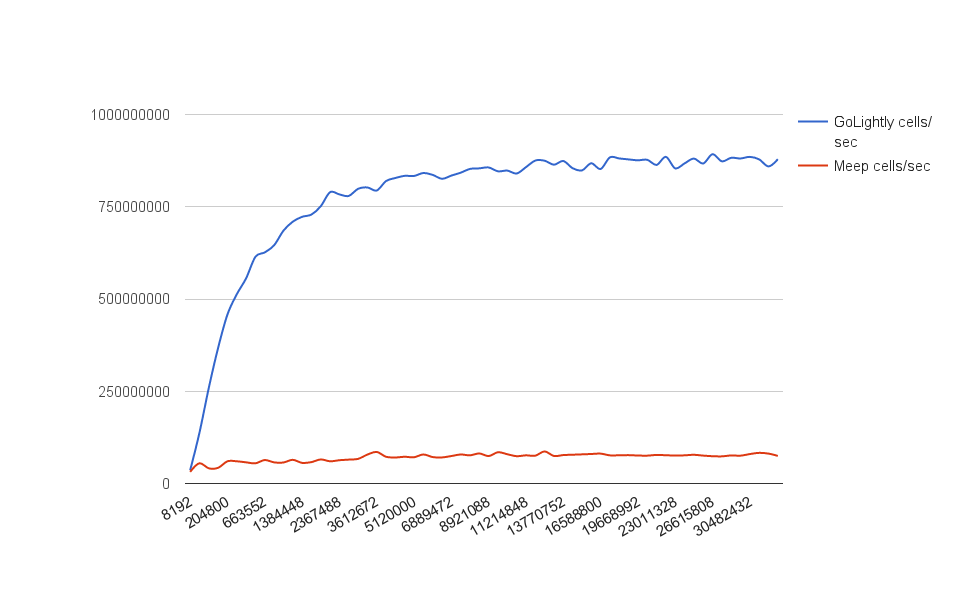
\includegraphics[width=\textwidth,
	keepaspectratio]{cells-per-second.png}
	\caption{GoLightly: Completed E and H updates per second}
	\label{fig:gridSizeVsComputeTime}
\end{figure}

Note that GPU throughput (represented in \autoref{fig:gridSizeVsComputeTime} as “cell” operations per second) increases dramatically as the domain size increases, until GPU initialization overhead is overcome by computation time.

Comparing to Meep:

\begin{figure}[H]
	\centering
	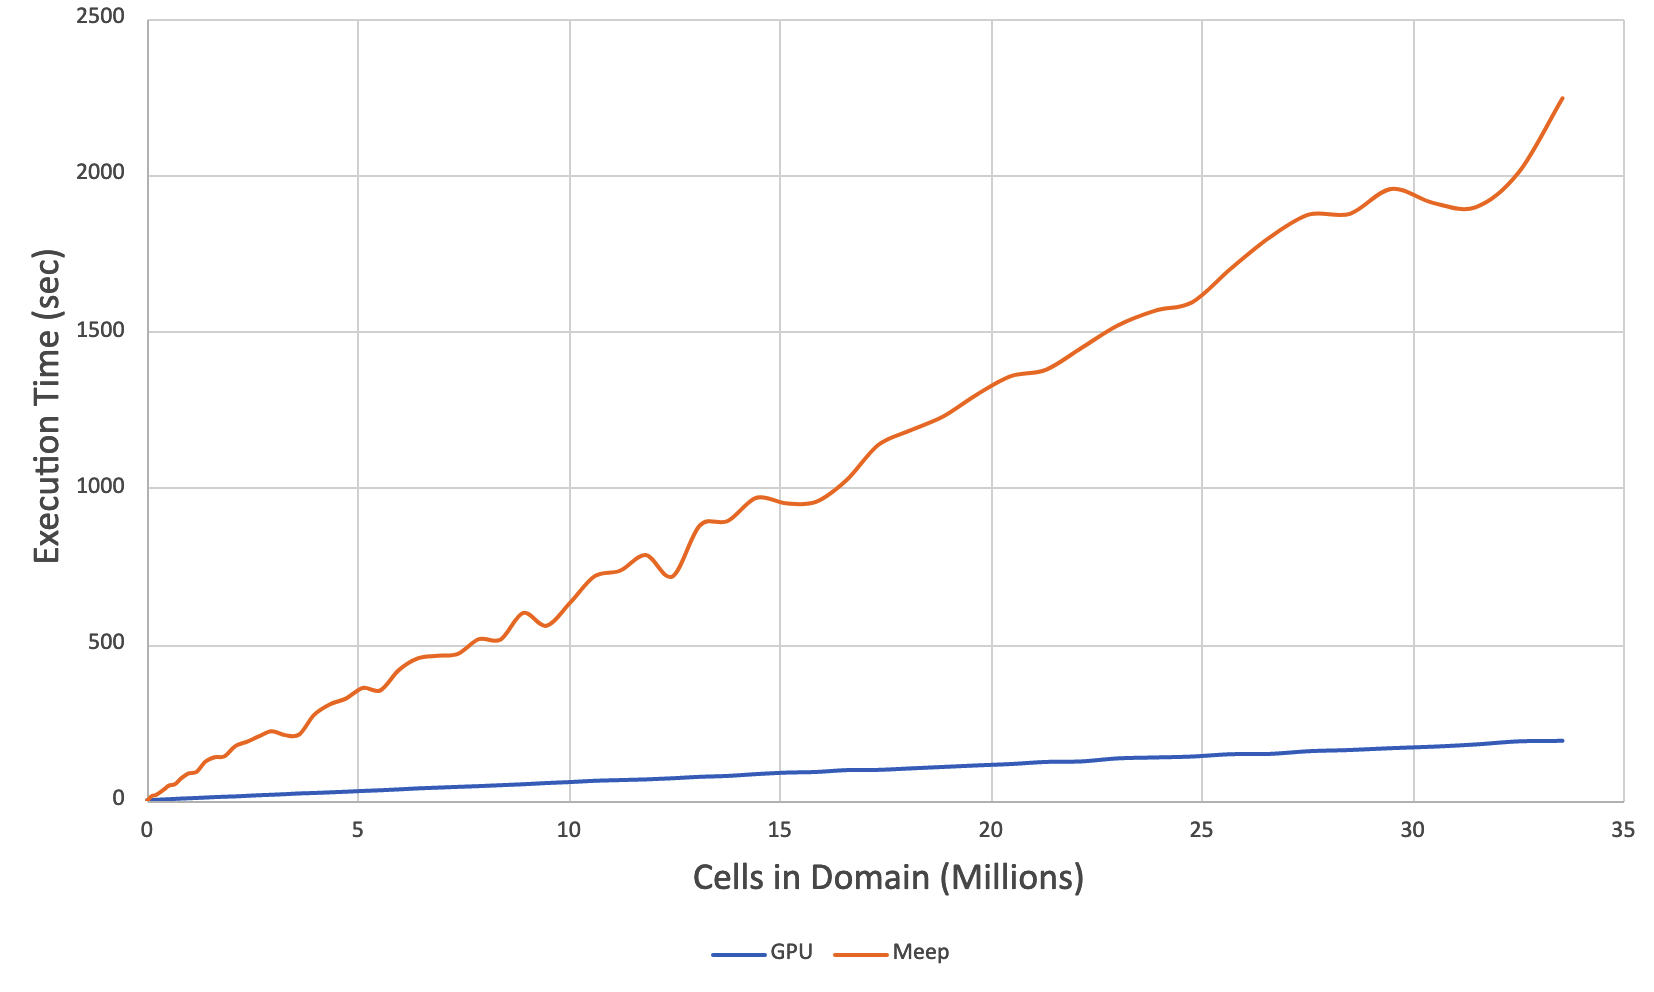
\includegraphics[width=\textwidth,
	keepaspectratio]{gpu-vs-meep.png}
	\caption{GoLightly vs Meep}
	\label{fig:gpuVsMeep}
\end{figure}

In \autoref{fig:gpuVsMeep}, note some CPU performance variance near the middle and end of the graph. Multiple runs consistently exhibited this behavior. While the cause of these variances is not clear, it has been reproduced on different hardware and operating system versions. Potential causes may include multitasking preemption, cache behavior for a given domain size, and others. See also \autoref{fig:gpuVsMeepSpeedup}.

\begin{figure}[H]
	\centering
	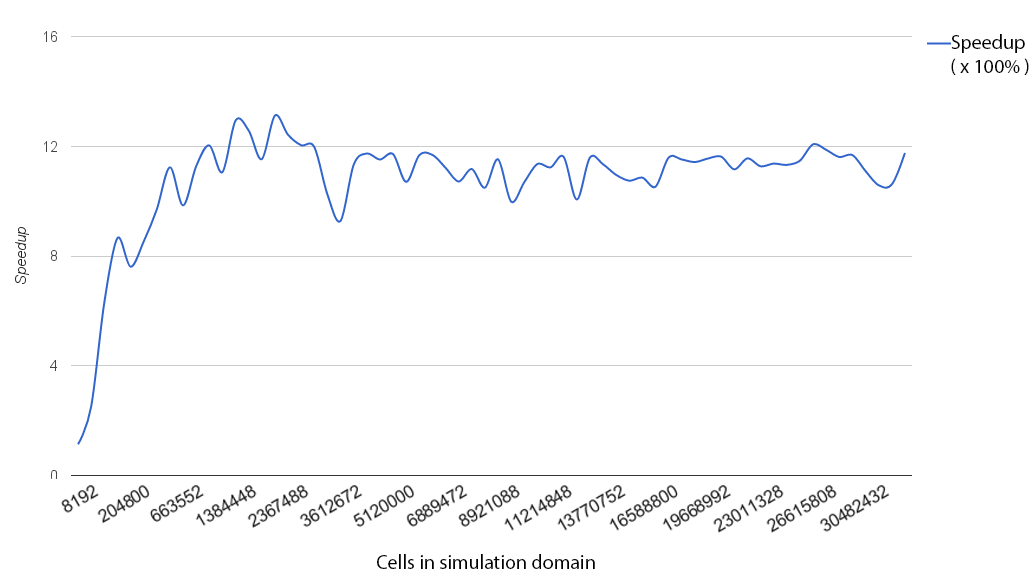
\includegraphics[width=\textwidth,
	keepaspectratio]{gpu-vs-meep-speedup.png}
	\caption{Speedup - Meep Time / GoLightly Time}
	\label{fig:gpuVsMeepSpeedup}
\end{figure}

This gives us a speedup ranging from 1.2 to 12, depending on the domain size. At lower resolutions, the overhead of initializing assets on the GPU can take more time than the simulation. In that case, the CPU may outperform the GPU solution.

\section{Optimization and Enhancements}

Although a 1200\% speed increase is significant, there is much room for improvement. 

GPUs provide different memory spaces that vary in size and access speed. In addition to global device memory, each warp (group of 32 threads sharing an ALU) has shared memory\footnote{Shared memory is physically local to the ALU and accessible by all threads within the warp.} and local memory\footnote{Each thread has local memory which is not accessible to any other thread}.

While global memory is the most flexible and plentiful - typically on the order of gigabytes on current generation hardware - it is also the slowest. 

Shared memory is roughly equivelant to a CPU's L2 cache. It can be used for intra-thread synchronization and resource sharing. It is significantly faster than global memory.

Finally, local memory - similar to a CPU L1 cache - provides thread-local storage. Local memory provides the lowest latency of all of the memory spaces.

In its current form, GoLightly makes little use of shared or local memory. Modifying the application to take advantage of those may improve performance.







